\documentclass[border=5pt]{standalone}

\usepackage{ifthen}

\usepackage{tikz}
\usetikzlibrary{calc, shapes}

\usepackage{mathpazo}

\def\circleDiameter{1}

\begin{document}
	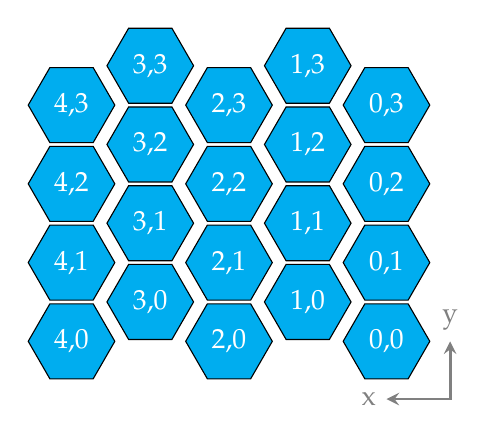
\begin{tikzpicture}
		\foreach \y in {0,1,2,3}{
			\foreach \x in {0,1,2,3,4}{
				\def\offsetX{0}
				\def\offsetY{0}
				\pgfmathparse{int(mod(\x,2))}
				\ifthenelse{\equal{\pgfmathresult}{1}}{
					\pgfmathsetmacro{\offsetY}{\circleDiameter/2}
				}{}
				\node[regular polygon, regular polygon sides=6, shape aspect=0.5, minimum width=1cm, minimum height=1cm, draw=black, fill=cyan, text=white] (node\x\y)
				at ($(\x*-\circleDiameter,\y*\circleDiameter)+(\offsetX, \offsetY)$) {\x,\y};
			}
		}
		
		\draw[<->, >=stealth, draw=gray, line width = 1pt]($(node00.south)+(0,-0.25)$)node[left, text=gray]{x}-|($(node00.east)+(0.25,0)$)node[above, text=gray]{y};
	\end{tikzpicture}
\end{document}